\documentclass[tikz,border=5pt,multi=tikzpicture]{standalone}
\usepackage[UTF8]{ctex}
\usepackage{amsmath}
\usetikzlibrary{arrows.meta,calc,decorations.markings}
\definecolor{ink}{HTML}{17365D}
\definecolor{field}{HTML}{287DA8}
\definecolor{force}{HTML}{C56B2A}
\tikzset{every node/.style={font=\small},vec/.style={-{Stealth[length=2mm]},thick},helper/.style={gray,dashed}}
\begin{document}
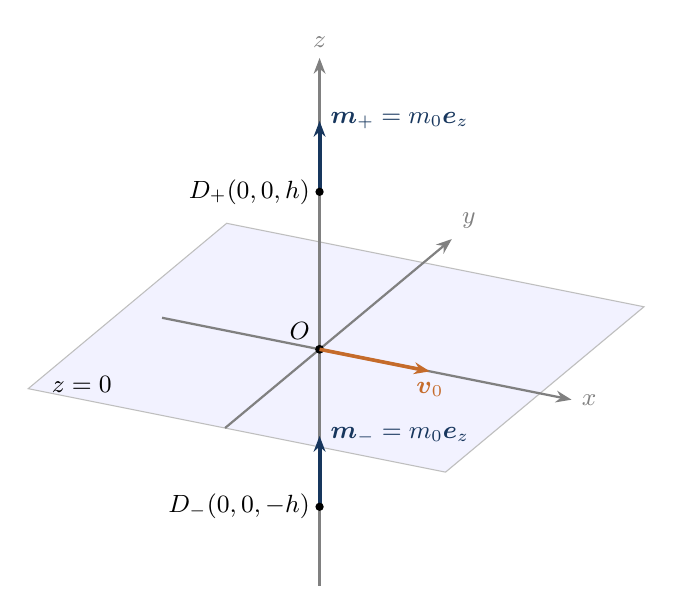
\begin{tikzpicture}[x={(1cm,-.20cm)},y={(.6cm,.5cm)},z={(0cm,1cm)}]
  \fill[blue!5] (-2.5,-2.0,0)--(2.8,-2.0,0)--(2.8,2.2,0)--(-2.5,2.2,0)--cycle;
  \draw[gray!50] (-2.5,-2.0,0)--(2.8,-2.0,0)--(2.8,2.2,0)--(-2.5,2.2,0)--cycle;
  \draw[vec,gray] (-2,0,0)--(3.2,0,0) node[right] {$x$};
  \draw[vec,gray] (0,-2,0)--(0,2.8,0) node[above right] {$y$};
  \draw[vec,gray] (0,0,-3.0)--(0,0,3.7) node[above] {$z$};
  \draw[vec,ink,line width=1.4pt] (0,0,2.0)--(0,0,2.9) node[right] {$\boldsymbol m_+=m_0\boldsymbol e_z$};
  \draw[vec,ink,line width=1.4pt] (0,0,-2.0)--(0,0,-1.1) node[right] {$\boldsymbol m_-=m_0\boldsymbol e_z$};
  \fill (0,0,2.0) circle (1.5pt) node[left] {$D_+(0,0,h)$};
  \fill (0,0,-2.0) circle (1.5pt) node[left] {$D_-(0,0,-h)$};
  \fill (0,0,0) circle (1.6pt) node[above left] {$O$};
  \draw[vec,force,line width=1.3pt] (0,0,0)--(1.4,0,0) node[below] {$\boldsymbol v_0$};
  \node at (-2,-1.7,0) {$z=0$};
\end{tikzpicture}
\begin{tikzpicture}
  \coordinate (O) at (0,0);\coordinate (P) at (2.2,0);
  \coordinate (Dplus) at (0,2);\coordinate (Dminus) at (0,-2);
  \draw[vec,gray] (-.5,0)--(4.7,0) node[right] {$r$};
  \draw[vec,gray] (0,-2.8)--(0,3.2) node[above] {$z$};
  \draw[helper] (Dplus)--(P)--(Dminus);
  \node[fill=white,inner sep=1pt] at (1.25,1.35) {$\sqrt{r^2+h^2}$};
  \node[fill=white,inner sep=1pt] at (1.25,-1.35) {$\sqrt{r^2+h^2}$};
  \draw[vec,ink] (Dplus)--++(0,.7) node[right] {$m_0$};
  \draw[vec,ink] (Dminus)--++(0,.7) node[left] {$m_0$};
  \fill (Dplus) circle (1.5pt) node[left] {$D_+$};
  \fill (Dminus) circle (1.5pt) node[left] {$D_-$};
  \fill (O) circle (1.2pt) node[below left] {$O$};
  \fill (P) circle (1.5pt) node[below right] {$P$};
  \draw[vec,field] (P)--++(-1.32,.316) node[above left] {$\boldsymbol B_+$};
  \draw[vec,field] (P)--++(1.32,.316) node[above right] {$\boldsymbol B_-$};
  \draw[vec,field,line width=1.3pt] (P)--++(0,.632) node[above] {$\boldsymbol B$};
  \node[align=left,anchor=west] at (5.4,1.5) {包含 $z$ 轴与 $P$ 的截面\\[4pt]两横向分量相消\\[4pt]两轴向分量相加\\[4pt]箭头示 $r<\sqrt2h$ 区域};
\end{tikzpicture}
\begin{tikzpicture}
  \draw[vec,gray] (-.6,0)--(4.6,0) node[right] {$x$};
  \draw[vec,gray] (0,-.8)--(0,3.6) node[above] {$y$};
  \coordinate (P) at (3,1.6);
  \draw[helper] (0,0)--(P);
  \draw[ink] (.8,0) arc (0:28.0725:.8) node[midway,right] {$\varphi$};
  \fill (0,0) circle (1.3pt) node[below left] {$O$};
  \fill (P) circle (1.7pt) node[above left] {$P$};
  \draw[vec,field] (P)--++(28.0725:1.25) node[right] {$v_r\boldsymbol e_r$};
  \draw[vec,field] (P)--++(-61.9275:1.15) node[below right] {$v_\varphi\boldsymbol e_\varphi$};
  \draw[ink] (4.4,3.1) circle (.11);\fill[ink] (4.4,3.1) circle (.035);
  \node[anchor=west] at (4.65,3.1) {$B_z>0$};
  \node at (2.0,4.15) {速度分解（$q>0$、$v_r>0$、$B_z>0$）};
  \begin{scope}[xshift=8.1cm,yshift=1.6cm]
    \draw[vec,gray] (0,0)--(28.0725:1.5) node[right] {$\boldsymbol e_r$};
    \draw[vec,gray] (0,0)--(118.0725:1.5) node[above left] {$\boldsymbol e_\varphi$};
    \draw[vec,force] (0,0)--(208.0725:1.15) node[below left] {$F_r<0$};
    \draw[vec,force] (0,0)--(298.0725:1.15) node[below right] {$F_\varphi<0$};
    \fill (0,0) circle (1.7pt);
    \node at (0,2.55) {同一位置的磁力分解};
  \end{scope}
\end{tikzpicture}
\begin{tikzpicture}[x=2.65cm,y=2.65cm]
  \draw[vec,gray] (0,0)--(3.0,0) node[right] {$r/h$};
  \draw[vec,gray] (0,0)--(0,1.8) node[above] {$W/v_c^2$};
  \draw[thick,ink,domain=0:2.8,samples=170] plot (\x,{6.75*\x*\x/(1+\x*\x)^3});
  \draw[helper] (.70710678,0)--(.70710678,1);
  \node[below] at (.70710678,0) {$1/\sqrt2$};
  \node[left] at (0,1) {$1$};
  \draw[thick,field] (0,1.44)--(2.8,1.44) node[right] {$v_0^2/v_c^2>1$};
  \draw[thick,force] (0,1)--(2.8,1) node[right] {$v_0^2/v_c^2=1$};
  \draw[thick,field,dashed] (0,.64)--(2.8,.64) node[right] {$v_0^2/v_c^2<1$};
  \fill (.70710678,1) circle (.025);
  \node[above,xshift=9pt] at (.70710678,1.03) {$r_b$};
  \node[align=left,anchor=west] at (3.5,.4) {$\dot r^2=v_0^2-W(r)$\\[4pt]从原点出发需越过峰顶};
\end{tikzpicture}
\end{document}
